\documentclass[conference]{IEEEtran}
\IEEEoverridecommandlockouts
\usepackage{amsmath,amssymb,amsfonts}
\usepackage{graphicx}
\usepackage{booktabs}
\usepackage{multirow}
\usepackage{array}
\usepackage{xcolor}
\usepackage{cite}
\usepackage[hidelinks]{hyperref}
\usepackage{siunitx}
\sisetup{detect-all}
\graphicspath{{fig/}}

\newcommand{\regen}{\ensuremath{\eta_{\mathrm{rg}}}}
\renewcommand{\arraystretch}{1.12}

\begin{document}

\title{Jackknife-Safe Regenerative Braking for a Battery-Electric Tractor--Semitrailer: Gain-Scheduled LQR Yaw Control with Friction-Circle-Constrained Brake Allocation}

\author{\IEEEauthorblockN{Roopesh Varun, Geoffrey, and Sivaranjani}
\IEEEauthorblockA{Department of Engineering Design, Indian Institute of Technology Madras, Chennai, India\\
ED5330 Control of Automotive Systems: Course Project, November 2026}}

\maketitle

\begin{abstract}
An electrified semitrailer axle gives an articulated truck a second axle for regenerative braking, but allocating braking for energy alone can saturate the tractor drive axle and jackknife the combination on low friction. This paper presents a controller that recovers braking energy on both units while keeping them yaw-stable. It combines three elements: a gain-scheduled linear quadratic regulator (LQR) on a four-state single-track model that demands corrective yaw moments on the tractor and semitrailer; a Kalman filter augmented with two yaw-moment disturbance states that estimates the unmeasured lateral velocity and articulation rate; and a new brake allocator that takes regeneration from the semitrailer first and caps each axle's braking so that it keeps the lateral grip the curve requires. The controller is evaluated on a nonlinear four-degree-of-freedom tractor--semitrailer model derived from Lagrange's equations with published parameters, over 77 simulations covering braking in a turn and a braked lane change, three payloads (13.5--39~t) and road friction from snow to dry asphalt. Energy-first allocation was unstable in 5 of 9 brake-in-turn cases, four of them full jackknifes. The proposed controller was stable in all 15 nominal manoeuvres and returned 73--77\% of the braking energy to the battery on snow, 19--26 percentage points more than the same LQR with energy-first allocation; an ablation shows that this gain comes from the allocator. The LQR raised trailer-sway damping at 30~m/s from 0.39 to 0.80. The only failure occurred when the payload was over-estimated, which makes a reliable, low-biased payload estimate a design requirement.
\end{abstract}

\begin{IEEEkeywords}
articulated heavy vehicles, regenerative braking, control allocation, yaw stability, jackknife, linear quadratic regulator, Kalman filter, electric semitrailer
\end{IEEEkeywords}

%======================================================================
\section{Introduction}

\subsection{Motivation}
Tractor--semitrailer combinations carry most long-haul road freight, and their electrification is under way. A battery-electric tractor can recover braking energy only through its drive axle. An electrified semitrailer axle, with its own motors connected to the vehicle battery, adds a second regenerative axle that usually carries more load than the tractor drive axle, and therefore more recoverable energy.

More regenerative axles create an allocation problem. A tyre's grip, approximately $\mu F_z$, is shared between braking and cornering. If the tractor drive axle is braked to its friction limit in a curve, it has no lateral force left; the rear of the tractor slides out and the tractor rotates towards the trailer, which is jackknife. Braking the semitrailer axle too hard causes the trailer to swing out in the same way. Both boundaries move with payload: an empty and an overloaded semitrailer differ several-fold in axle load. On roads where overloading beyond the rated payload is common, a controller tuned for one load is not sufficient. Fig.~\ref{fig:paths} previews the failure this paper addresses.

\subsection{Literature Review}
The Chalmers--Volvo group has studied this problem most directly. Erdinc \emph{et al.}~\cite{erdinc2023} built a two-track model of a tractor--semitrailer and computed a safe operating envelope (SOE) over \num{40804} brake combinations at $\mu=0.3$, defining instability as a side-slip deviation of \ang{5} at the tractor drive axle and \ang{3} at the semitrailer axle. The SOE is a static map, not a feedback controller. Erdin\c{c}~\cite{erdinc2024thesis} allocated propulsion and regeneration between tractor and semitrailer to minimise power loss within the SOE and slip limits, and showed in brake-in-turn tests that loss-minimising allocation without safety constraints jackknifes on low friction; by the author's own statement the allocation is instantaneous, uses longitudinal forces only and has no yaw feedback. Erdinc \emph{et al.}~\cite{erdinc2024avec} shrank the motor slip limit as the tractor side-slip deviated from its reference (a ``slip polytope''), keeping side-slip below \ang{2} on ice where a fixed limit failed, but used only tractor states.

A second line of work uses semitrailer actuators for stability without an energy objective. Bai \emph{et al.}~\cite{bai2020} added hub motors to the semitrailer and used a fuzzy-PID yaw-moment controller with wheel-torque distribution, improving lateral stability over differential braking in TruckSim, for a single payload. Vignati \emph{et al.}~\cite{vignati2020} stabilised a car--trailer up to 140~km/h with torque vectoring on the towing car, with the benefit ending at motor saturation. Optimal control has also been applied to articulated trucks: Hou and Xu~\cite{hou2022} used LQR to steer the trailer's middle axle, and Deng \emph{et al.}~\cite{deng2026} combined LQR rear-axle steering with a linear time-varying model predictive yaw-moment controller on a distributed-drive electric tractor--semitrailer; neither treats regenerative braking or energy recovery. Supporting work includes online vehicle-mass estimation by recursive least squares~\cite{vahidi2005}, motor-based slip control for electric vehicles~\cite{ivanov2015}, which justifies treating wheel forces as tracked within the friction limit, the single-track lateral model~\cite{rajamani2012}, and the absence of guaranteed stability margins for LQG regulators~\cite{doyle1978}.

\subsection{Research Gap}
Published work either stabilises the semitrailer with motors or steering without optimising energy~\cite{bai2020,vignati2020,hou2022,deng2026}, or allocates braking for energy with an instantaneous safety layer and no yaw feedback~\cite{erdinc2024thesis,erdinc2024avec}. In the literature reviewed, no work closes a yaw feedback loop on both the tractor and the semitrailer while allocating regenerative braking between them for energy, and none quantifies how such a scheme behaves across payload and payload-estimation error.

\subsection{Novelty and Contributions}
This paper makes four contributions:
\begin{enumerate}
\item A closed-loop scheme that couples gain-scheduled LQR yaw feedback on both units with a \emph{semitrailer-first, friction-circle-capped} regenerative brake allocator for an electrified semitrailer, which respects motor, battery and open-differential constraints.
\item A quantified stability--energy trade-off over three payloads and three road frictions against three baselines, including an ablation that isolates the allocator's contribution.
\item Two estimation results for the tractor--semitrailer: with load-proportional cornering stiffness, a lateral drift mode is unobservable from yaw rate and articulation angle but stable (detectable); and a disturbance-augmented Kalman filter removes the articulation-rate bias caused by braking, but is not detectable with yaw rate alone.
\item An asymmetric robustness finding: under-estimating the payload is safe but costs energy, while over-estimating it is the one failure mode found.
\end{enumerate}

%======================================================================
\section{Modelling and Methodology}

The method has five steps (Fig.~\ref{fig:arch}): a nonlinear plant model, a linear design model, estimation and LQR control, the stability-capped allocator, and simulation-based evaluation. The nonlinear model plays the role of the real vehicle; the controller sees only noisy yaw rate and articulation angle.

\begin{figure*}[t]
\centering
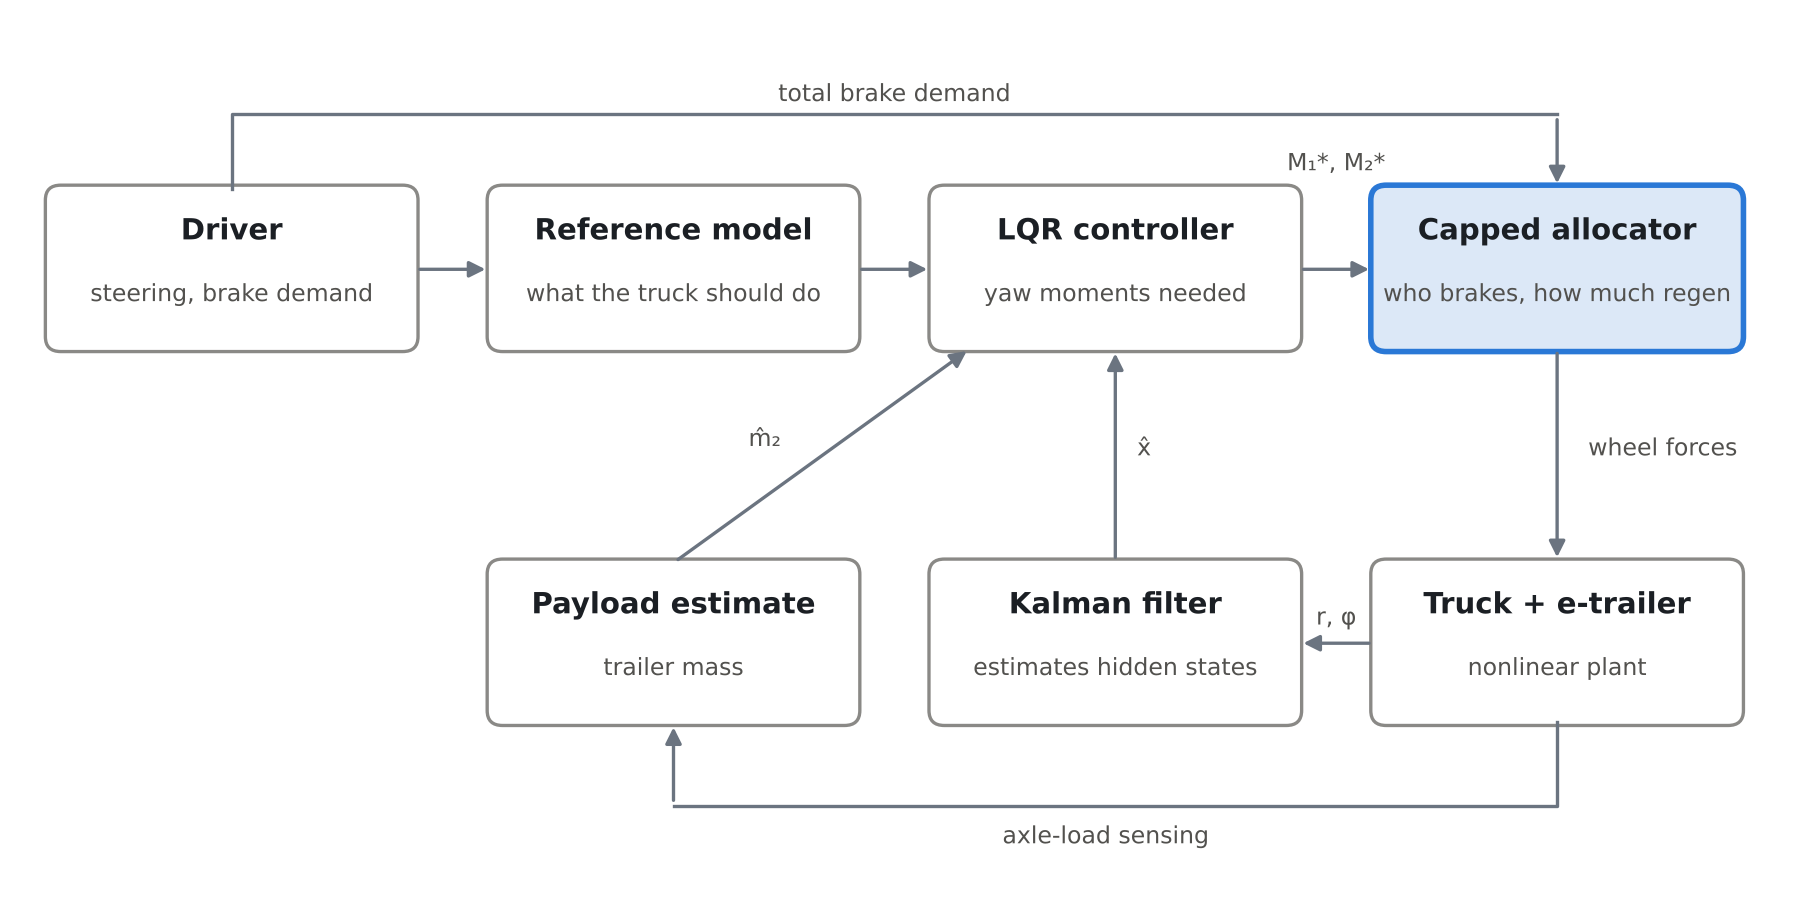
\includegraphics[width=0.78\textwidth]{architecture.png}
\caption{Closed-loop architecture. Every \SI{10}{ms} the Kalman filter estimates the state, the reference model and gain-scheduled LQR compute the tractor and semitrailer yaw moments $M_1,M_2$, and the proposed allocator (highlighted) converts the driver's brake demand and these moments into six wheel forces, regenerative where safe. The nonlinear plant is integrated by RK4 at \SI{5}{ms}.}
\label{fig:arch}
\end{figure*}

\subsection{Vehicle}
A $4\times2$ battery-electric tractor (steer axle; drive axle with one e-axle motor and an open differential) pulls a semitrailer whose axle group, lumped as one axle, has independent left and right motors. All wheels have slip-controlled friction brakes. Geometry, masses, inertias, centre-of-gravity (CoG) heights, track width and tyre cornering stiffness are taken from~\cite{erdinc2023} (Fig.~\ref{fig:layout}, Table~\ref{tab:params}). Three semitrailer payloads are studied: light (13.5~t, the published value), rated (30~t) and overloaded (39~t, rated $+30\%$); for the heavier payloads the semitrailer mass and yaw inertia are scaled together with the CoG kept in place.

\begin{figure}[t]
\centering
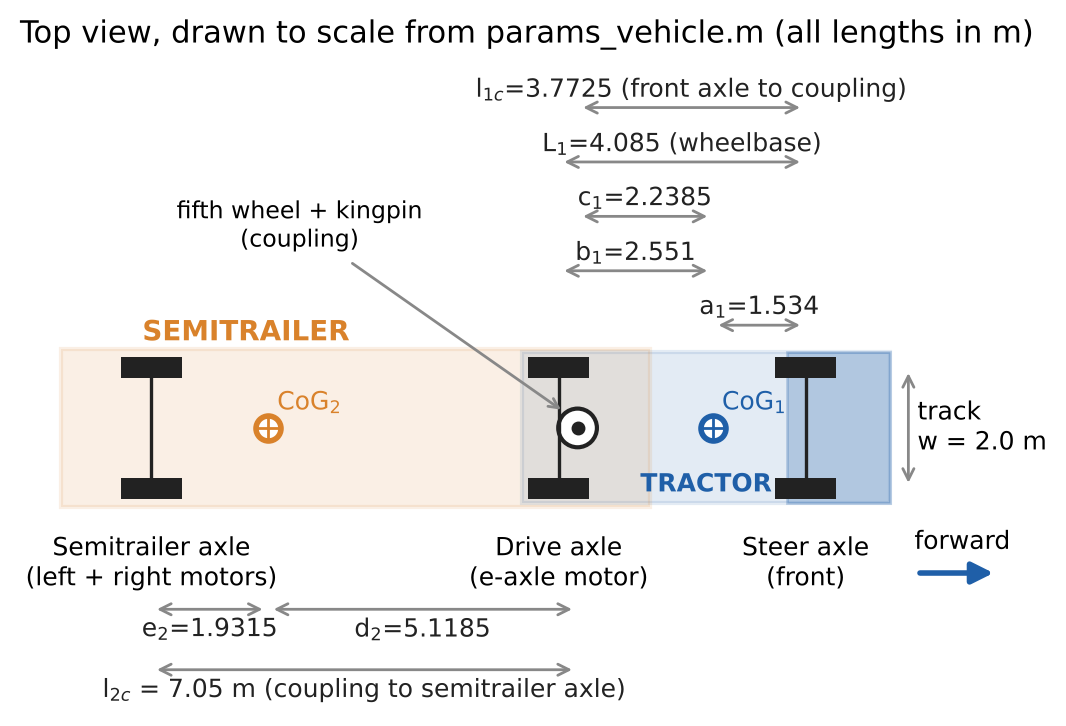
\includegraphics[width=\columnwidth]{f01_layout_top.png}
\caption{Top view of the tractor--semitrailer drawn to scale from the parameters, with the steer, drive and semitrailer axles, the two CoGs and the coupling.}
\label{fig:layout}
\end{figure}

\subsection{Nonlinear Planar Model}
The generalised coordinates are $q=[X,\,Y,\,\psi_1,\,\varphi]^\top$: the tractor CoG position, the tractor heading and the articulation angle, with semitrailer heading $\psi_2=\psi_1-\varphi$. Two rigid bodies in the plane have six degrees of freedom; the coupling removes two, leaving four. With unit vectors $\mathbf e_i=[\cos\psi_i,\ \sin\psi_i]^\top$, the coupling point and semitrailer CoG are
\begin{equation}
\mathbf p_h=\mathbf p_1-c_1\mathbf e_1,\qquad \mathbf p_2=\mathbf p_h-d_2\mathbf e_2,
\end{equation}
where $c_1$ is the tractor CoG-to-coupling distance and $d_2$ the coupling-to-semitrailer-CoG distance. On a flat road the Lagrangian equals the kinetic energy,
\begin{equation}
T=\tfrac12 m_1\|\dot{\mathbf p}_1\|^2+\tfrac12 I_1\dot\psi_1^2+\tfrac12 m_2\|\dot{\mathbf p}_2\|^2+\tfrac12 I_2\dot\psi_2^2,
\end{equation}
and Lagrange's equations
\begin{equation}
\frac{d}{dt}\frac{\partial T}{\partial \dot q_i}-\frac{\partial T}{\partial q_i}=Q_i,\qquad
Q_i=\sum_a \mathbf F_a\cdot\frac{\partial \mathbf p_a}{\partial q_i}+\sum_b M_b\frac{\partial\psi_b}{\partial q_i}
\end{equation}
give the generalised forces from each axle force $\mathbf F_a$ (rotated from its body frame) acting at axle point $\mathbf p_a(q)$, and from each left--right yaw moment $M_b=\tfrac{w}{2}(F_{x,R}-F_{x,L})$ on body $b$. The equations were derived symbolically in SymPy and exported to MATLAB in the form
\begin{equation}
M(q)\,\ddot q=h(q,\dot q,\mathbf F),
\end{equation}
which is solved for $\ddot q$ at each evaluation and integrated by fourth-order Runge--Kutta (RK4) at \SI{5}{ms}. Minimal coordinates enforce the coupling constraint exactly, with no constraint drift. The yaw entry of the mass matrix,
\begin{equation}
M_{33}=I_1+I_2+m_2\left(c_1^2+2c_1d_2\cos\varphi+d_2^2\right),
\end{equation}
is the combination's yaw inertia about the tractor CoG (\SI{863400}{kg\,m^2} at $\varphi=0$, light payload). The generalised force on $\psi_1$ contains the term $c_1\sin\varphi\,F_{xt}$: when the vehicle is articulated, semitrailer braking ($F_{xt}<0$) produces a moment that straightens the combination.

\subsection{Tyre and Axle-Load Models}
Each wheel's lateral force follows the tanh law with a friction-circle reduction, the structure used in~\cite{erdinc2023}:
\begin{equation}
F_{y0}=-\mu F_z\tanh\!\left(\frac{C_n\alpha}{\mu}\right),\quad
F_y=F_{y0}\sqrt{1-\left(\frac{F_x}{\mu F_z}\right)^2},
\label{eq:tyre}
\end{equation}
with $C_n=\SI{6}{rad^{-1}}$, so the cornering stiffness $C_nF_z$ is proportional to load. A wheel braking at its friction limit ($|F_x|=\mu F_z$) has no lateral capacity left; this is the mechanism of jackknife and trailer swing. Slip angles are computed from the body-frame velocities at each axle, e.g.\ $\alpha_r=\arctan\!\big((v_{y1}-b_1r_1)/v_{x1}\big)$ at the drive axle. Longitudinal wheel forces are clipped to $\pm\mu F_z$, standing in for slip-controlled brakes and motors~\cite{ivanov2015}.

Axle loads include quasi-static longitudinal load transfer from two side-view moment balances, about the semitrailer axle contact point and the tractor front-axle contact point. With deceleration $a_x<0$ and semitrailer braking force $F_{xt}$, the coupling forces and the drive-axle load are
\begin{align}
F_{cx}&=m_2a_x-F_{xt},\\
F_{cz}&=\left(e_2m_2g-h_2m_2a_x+h_cF_{cx}\right)/l_{2c},\\
F_{zr}&=\left(a_1m_1g+h_1m_1a_x+l_{1c}F_{cz}+h_cF_{cx}\right)/L_1,
\end{align}
and the semitrailer and front loads follow from vertical equilibrium. At \SI{1.03}{m/s^2} deceleration the drive-axle load falls from \SI{71.3}{kN} to \SI{65.3}{kN} when the tractor brakes alone, but rises to \SI{72.8}{kN} when the semitrailer supplies \SI{19.9}{kN} of the braking, a second physical reason to brake the semitrailer first. Lateral load transfer is not modelled.

\subsection{Linear Design Model}
At constant speed $u$, with small angles and linear tyres ($C_f,C_r,C_t$ equal to $C_n$ times the static axle loads), the state is $x=[v_1,\,r_1,\,\dot\varphi,\,\varphi]^\top$ (tractor lateral velocity, tractor yaw rate, articulation rate and angle), and the inputs are the control yaw moments $M_1,M_2$ and the steer angle $\delta$:
\begin{align}
m_1(\dot v_1+ur_1)&=F_{yf}+F_{yr}-F_h,\\
I_1\dot r_1&=a_1F_{yf}-b_1F_{yr}+c_1F_h+M_1,\\
m_2(\dot v_2+ur_2)&=F_{yt}+F_h,\\
I_2\dot r_2&=d_2F_h-e_2F_{yt}+M_2,
\end{align}
with $v_2=v_1-c_1r_1-d_2r_2+u\varphi$ and $r_2=r_1-\dot\varphi$. Eliminating the hitch force $F_h$ (in SymPy) gives
\begin{equation}
\dot x=A(u)\,x+B(u)\,[M_1,\ M_2,\ \delta]^\top .
\end{equation}

\subsection{Model Verification and Structural Properties}
Table~\ref{tab:checks} summarises the checks. The linear and nonlinear models agree to five significant figures for a small steer input; for a large steer on snow the nonlinear yaw rate is 8\% lower because its tyres saturate (Fig.~\ref{fig:linnl}). At low speed the yaw rate equals the kinematic value $u\delta/L_1$. The open-loop sway pair has damping ratio 0.96, 0.59 and 0.39 at 10, 20 and \SI{30}{m/s}.

The pair $(A,[B_{M_1}\ B_{M_2}])$ is controllable at every speed and payload, and remains controllable with the semitrailer moment alone. With a yaw-rate gyro and an articulation-angle sensor, however, the observability rank is 3 of 4. The first column of $A$ is $[-C_ng/u,\,0,\,0,\,0]^\top$: because cornering stiffness is proportional to load, every axle resists a uniform sideways drift in proportion to the weight it carries, so the drift produces no yaw moment on either unit and is invisible to rotation sensors. Its eigenvalue $-C_ng/u$ ($\SI{-2.94}{s^{-1}}$ at \SI{20}{m/s}, independent of payload) is stable, so the pair is detectable and a Kalman filter converges. A lateral accelerometer would restore full rank.

\begin{table}[t]
\caption{Model Checks (Light Payload)}
\label{tab:checks}
\centering
\begin{tabular}{@{}p{3.9cm}p{4.0cm}@{}}
\toprule
Check & Result\\
\midrule
Linear vs nonlinear, \SI{15}{m/s}, \SI{0.005}{rad} steer, \SI{3}{s} & $r_1$: 0.01835 vs 0.01835 rad/s; $\varphi$: 0.00824 vs 0.00824 rad\\
Large steer, $\mu=0.3$, \SI{0.06}{rad} & $r_1$: 0.220 (linear) vs 0.204 rad/s\\
Kinematic limit, \SI{5}{m/s}, \SI{0.05}{rad} & $r_1=0.0612$ rad/s $=u\delta/L_1$\\
Open-loop eigenvalues, 5--30 m/s & all in left half-plane\\
Controllability, $[M_1,M_2]$ / $M_2$ only & rank 4 / rank 4\\
Observability, $r_1$+$\varphi$ & rank 3 (drift mode, stable)\\
Observability, $r_1$+$a_y$ & rank 4\\
\bottomrule
\end{tabular}
\end{table}

\begin{figure}[t]
\centering
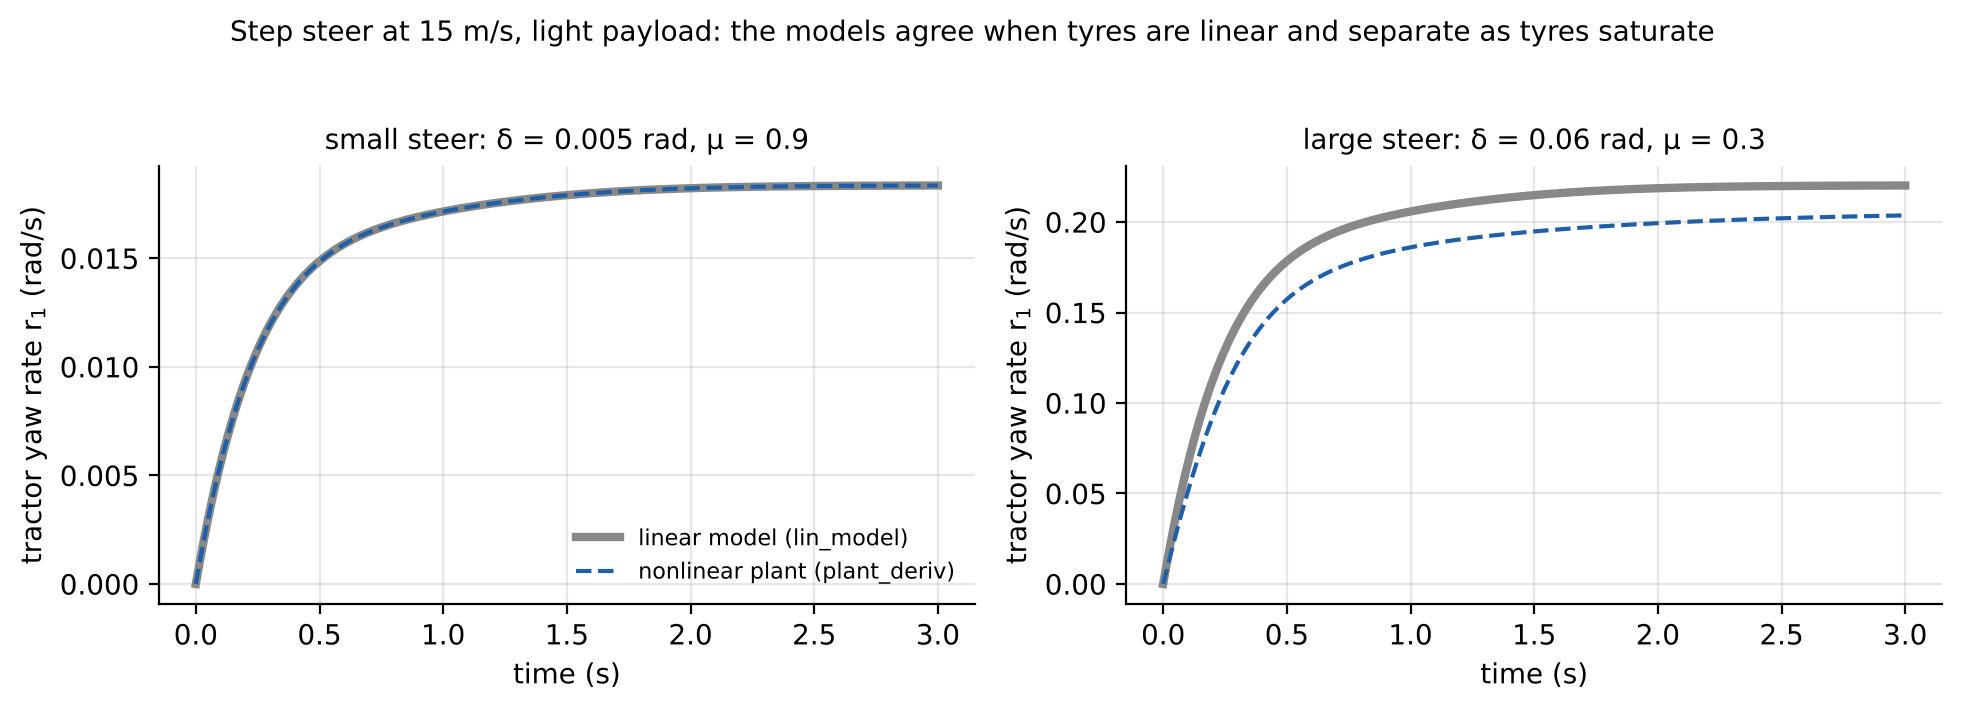
\includegraphics[width=\columnwidth]{f13_lin_vs_nonlin.png}
\caption{Step-steer response at \SI{15}{m/s}: linear and nonlinear yaw rates coincide for a small steer (left) and separate by about 8\% for a large steer on snow (right), where the nonlinear tyres saturate.}
\label{fig:linnl}
\end{figure}

\subsection{Reference Model}
The desired state is the linear model's steady-state response to the current steer at the current speed, scaled down so that the implied lateral acceleration does not exceed 85\% of the friction limit:
\begin{equation}
x_{\mathrm{ref}}=-A(u)^{-1}B_\delta(u)\,\delta,\qquad |u\,r_{1,\mathrm{ref}}|\le 0.85\,\mu g .
\end{equation}

\subsection{Gain-Scheduled LQR}
With control input $u_c=[M_1,M_2]^\top$ and error $e=\hat x-x_{\mathrm{ref}}$, the LQR minimises
\begin{equation}
J=\int_0^\infty\left(e^\top Qe+u_c^\top Ru_c\right)dt,
\end{equation}
giving $u_c=-Ke$ with $K=R^{-1}B_u^\top S$, where $S$ solves the algebraic Riccati equation
\begin{equation}
A^\top S+SA-SB_uR^{-1}B_u^\top S+Q=0 .
\end{equation}
The weights follow Bryson's rule, $Q=\mathrm{diag}(1/x_{\max}^2)$ with $x_{\max}=[\SI{0.3}{m/s},\SI{0.02}{rad/s},\SI{0.03}{rad/s},\SI{0.01}{rad}]$ and $R=\mathrm{diag}(1/u_{\max}^2)$ with $u_{\max}=\SI{30}{kN\,m}$, so the articulation angle receives the largest weight. The Riccati equation is solved from the stable eigenvectors of the Hamiltonian matrix $\left[\begin{smallmatrix}A & -B_uR^{-1}B_u^\top\\ -Q & -A^\top\end{smallmatrix}\right]$ as $S=X_2X_1^{-1}$, without toolbox dependencies. Gains are computed on a speed grid from 3 to \SI{30}{m/s} for the payload the controller assumes and interpolated linearly in measured speed; moments are limited to $\pm\SI{60}{kN\,m}$. At \SI{20}{m/s} the closed-loop poles are $-35.4$, $-3.51$ and $-3.03\pm1.66j$, and at \SI{30}{m/s} the sway damping rises from 0.39 to 0.80 (Fig.~\ref{fig:poles}). Because the scheduled LQR is combined with a Kalman filter, the loop is an LQG design without guaranteed margins~\cite{doyle1978}; robustness is therefore assessed by simulation (Section~\ref{sec:robust}).

\begin{figure}[t]
\centering
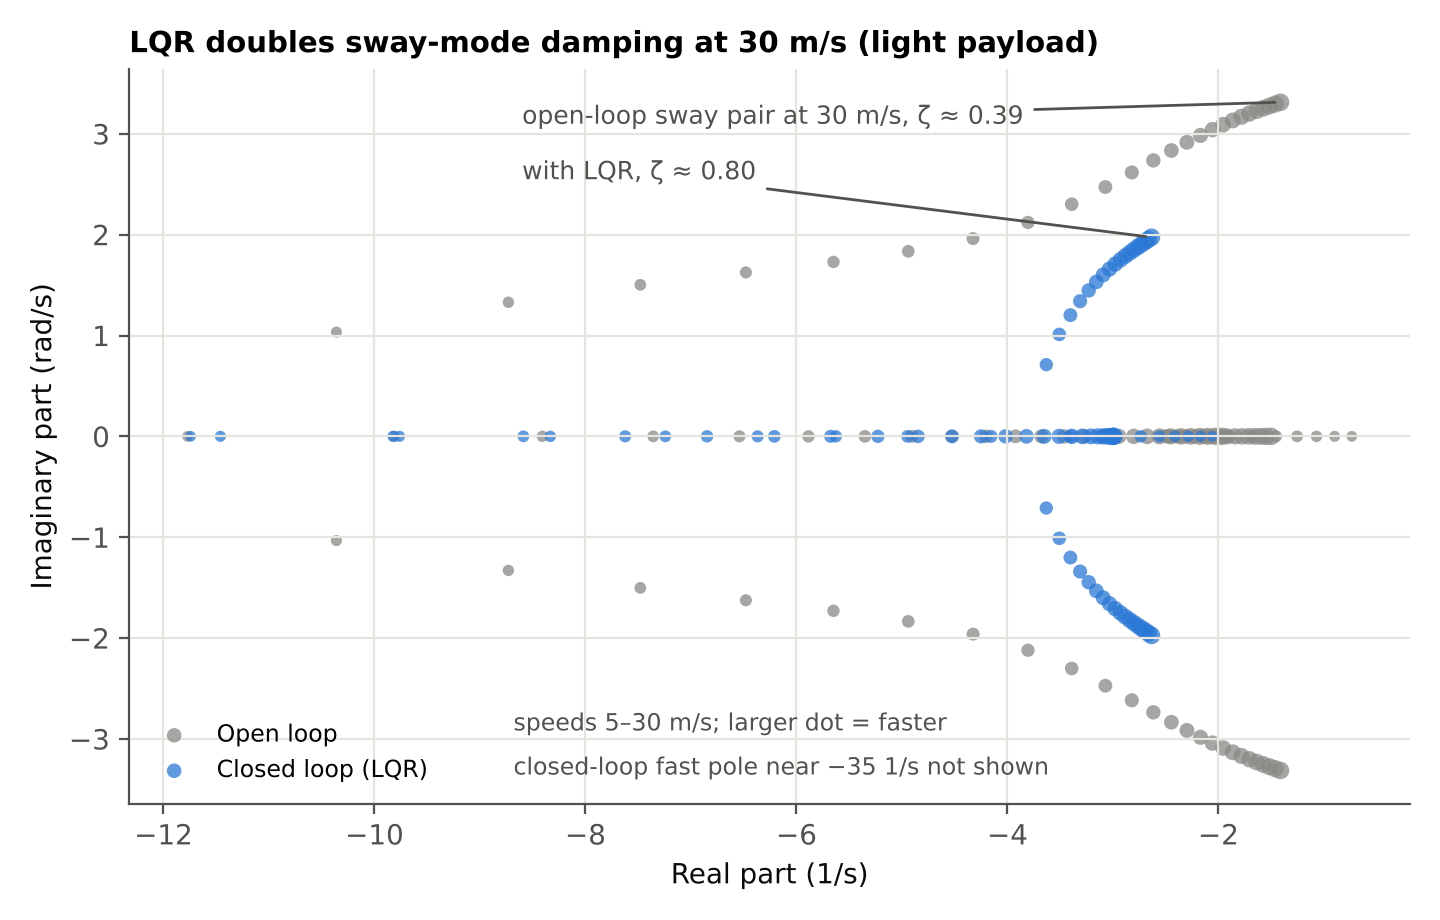
\includegraphics[width=\columnwidth]{fig5_poles.png}
\caption{Poles of the design model from 5 to \SI{30}{m/s} (light payload) without and with LQR. The LQR moves the sway pair from $\zeta\approx0.39$ to $\zeta\approx0.80$ at \SI{30}{m/s}.}
\label{fig:poles}
\end{figure}

\subsection{Disturbance-Augmented Kalman Filter}
The sensors are a yaw-rate gyro ($\sigma=\SI{0.003}{rad/s}$) and an articulation-angle sensor ($\sigma=\SI{0.005}{rad}$). A first filter on the four-state model gave a biased articulation-rate estimate during braking, of about \SI{1.5}{\degree/s}: unequal braking of the two units at an angle creates a yaw coupling that the linear model does not contain. The filter was therefore augmented with two random-walk yaw-moment disturbances $d=[d_1,d_2]^\top$ that enter through the same channels as $M_1,M_2$:
\begin{equation}
\begin{bmatrix}\dot x\\ \dot d\end{bmatrix}=
\begin{bmatrix}A & B_u\\ 0 & 0\end{bmatrix}\!
\begin{bmatrix}x\\ d\end{bmatrix}+
\begin{bmatrix}B\\ 0\end{bmatrix}\!
\begin{bmatrix}M_1\\ M_2\\ \delta\end{bmatrix}+w,\quad
y=\begin{bmatrix}r_1\\ \varphi\end{bmatrix}+v .
\end{equation}
The model is re-discretised every step at the measured speed by the matrix exponential (zero-order hold, \SI{10}{ms}), and its inputs are the yaw moments \emph{commanded} at the wheels in the previous step, since wheel limits can clip the LQR demand. The augmented pair has observability rank 5 of 6 with both sensors; the missing mode is the stable drift, so it is detectable. With the yaw-rate gyro alone the rank drops to 4 of 6 and a random-walk disturbance becomes unobservable with eigenvalue zero, which is not detectable; that sensor set therefore uses the plain four-state filter. In the snow brake-in-turn, the augmented filter's articulation-rate estimate after brake onset has a mean error of \SI{0.07}{\degree/s} and an RMS error of \SI{0.4}{\degree/s} (Fig.~\ref{fig:kf}).

\subsection{Stability-Constrained Brake Allocation (Proposed)}
For each axle $a\in\{$front, drive, semitrailer$\}$ with estimated load $F_{z,a}$, the braking the axle may carry is capped so that it keeps the lateral force the curve needs:
\begin{equation}
B_{a,\max}=\sqrt{\left(s_a\mu F_{z,a}\right)^2-\left(F_{z,a}\,a_y/g\right)^2},
\label{eq:cap}
\end{equation}
with safety factors $s=[0.90,\,0.70,\,0.85]$. The drive axle receives the tightest factor because its saturation initiates jackknife. Motor force limits are $\min(F_{\max},P_{\max}/v)$ per motor and the battery limit is $P_{\mathrm{bat}}/v$ on the total regenerative force. The brake demand $D$ is filled in this order:
\begin{enumerate}
\item semitrailer regeneration, up to its cap, the two motors' force and power limits and the battery limit;
\item tractor drive-axle regeneration, within its cap and the same limits;
\item friction braking on the steer axle, then the semitrailer, then the drive axle, each up to its cap;
\item if demand remains (an emergency stop), friction braking on all axles up to the full friction limit, so the driver's demand always has priority.
\end{enumerate}
The yaw moments are realised by left--right splits on each axle,
\begin{equation}
B_{a,L}=\frac{B_a}{2}+\frac{M_a}{w},\qquad B_{a,R}=\frac{B_a}{2}-\frac{M_a}{w},
\end{equation}
with $M_1$ shared between the steer and drive axles in proportion to load. The semitrailer motors are independent, so they can generate a moment regeneratively. The tractor's single motor with an open differential gives equal force to both wheels, so its motor force is limited to the smaller wheel demand and any tractor moment is produced by friction. Fig.~\ref{fig:alloc} shows the allocators at one instant on snow: energy-first allocation places \SI{19.6}{kN} on the drive axle, its entire friction limit, whereas the proposed allocator places \SI{19.9}{kN} on the semitrailer and \SI{4.6}{kN} on the drive axle while still sending all of it to the battery.

\begin{figure*}[t]
\centering
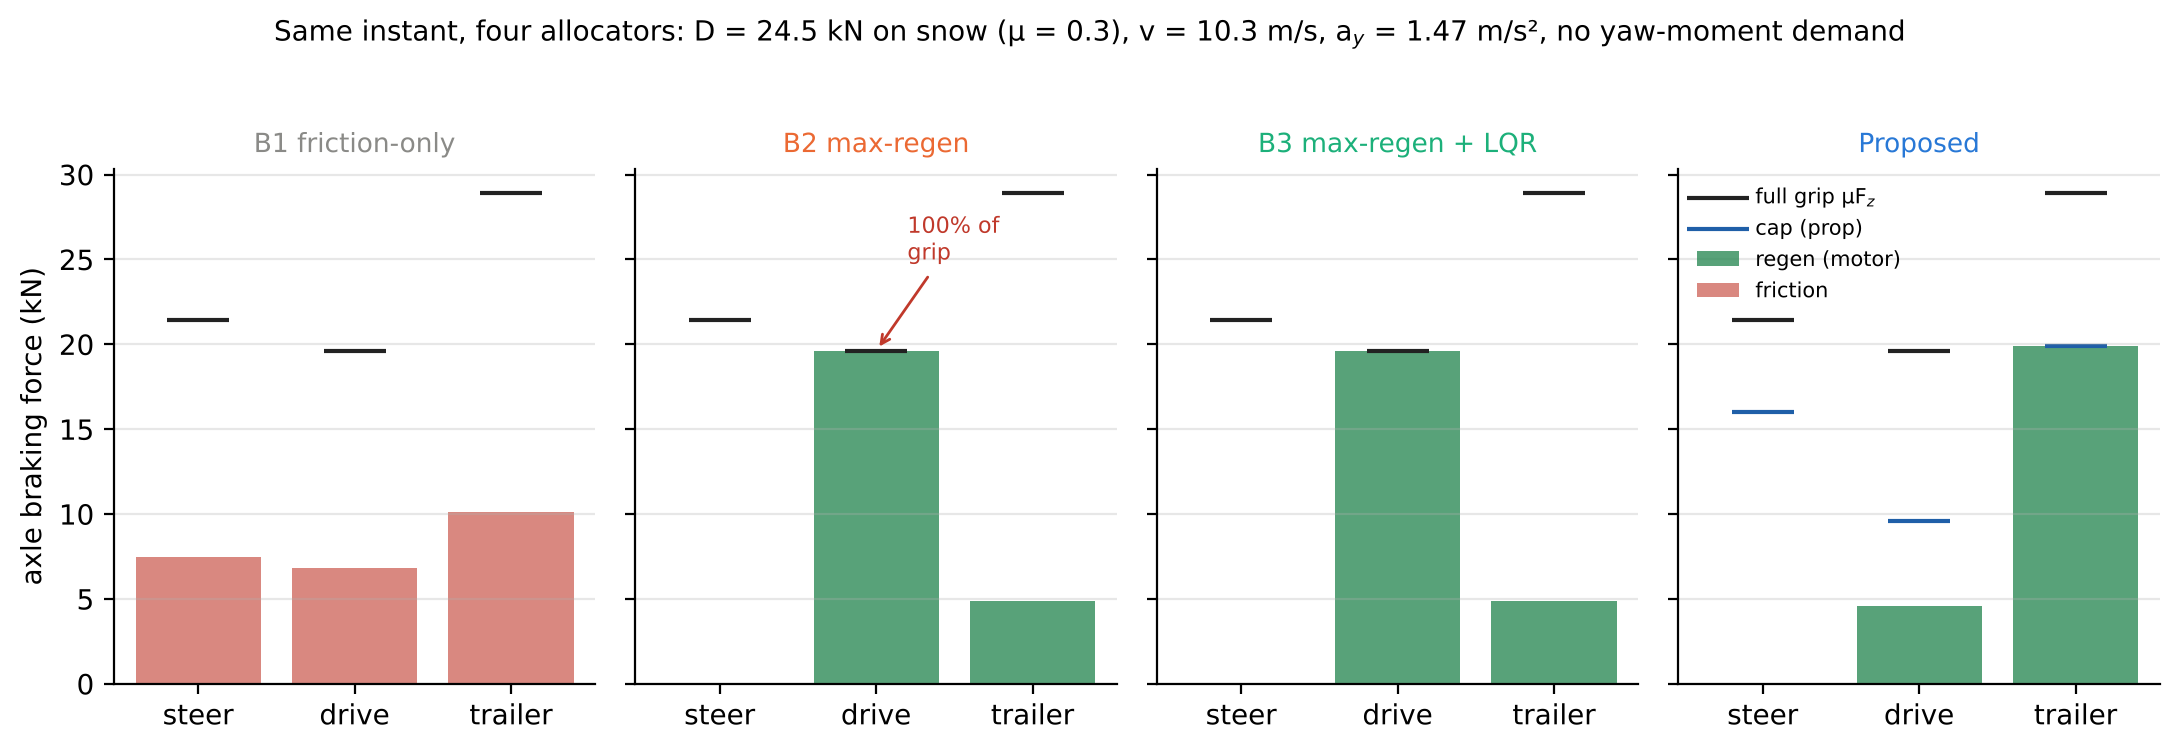
\includegraphics[width=0.92\textwidth]{g10_alloc_example.png}
\caption{Allocation of the same \SI{24.5}{kN} brake demand on snow ($\mu=0.3$, \SI{10.3}{m/s}, $a_y=\SI{1.47}{m/s^2}$). Axle caps from \eqref{eq:cap}: 16.0, 9.6 and \SI{19.9}{kN}. Energy-first allocation (B2) uses 100\% of the drive axle's grip; the proposed allocator moves the regeneration to the semitrailer.}
\label{fig:alloc}
\end{figure*}

\subsection{Baseline Controllers}
Three baselines isolate the contribution of each element (Table~\ref{tab:baselines}). B3 is the ablation: it shares the proposed controller's reference model, LQR and Kalman filter and differs only in the allocator.

\begin{table}[t]
\caption{Controllers Compared}
\label{tab:baselines}
\centering
\begin{tabular}{@{}lp{3.5cm}l@{}}
\toprule
Name & Brake allocation & Yaw control\\
\midrule
B1 & Friction only, by axle load & LQR\\
B2 & Max.\ regeneration, drive axle first, then semitrailer & None\\
B3 & As B2 & LQR\\
Proposed & Capped, semitrailer first & LQR\\
\bottomrule
\end{tabular}
\end{table}

%======================================================================
\section{Simulation Setup}

\subsection{Implementation}
All models and controllers are written as MATLAB-compatible functions. The plant is integrated by RK4 at \SI{5}{ms}; the controller and estimator run at \SI{10}{ms} with wheel forces held between updates. Speed and filtered deceleration are assumed measured exactly, and road friction is assumed known to the allocator. Sensor noise is Gaussian with a fixed seed. The results were produced with GNU Octave 8.4. A Simulink model is generated by script, with each block a MATLAB Function block calling the same functions; executing these blocks in order without Simulink reproduces the script results exactly (identical battery energy to six decimals for the proposed controller, B1 and B2 on snow). Table~\ref{tab:params} lists the parameters.

\begin{table}[t]
\caption{Parameters}
\label{tab:params}
\centering
\begin{tabular}{@{}p{3.6cm}p{2.6cm}l@{}}
\toprule
Parameter & Value & Source\\
\midrule
Tractor mass; yaw inertia & \SI{10250}{kg}; \SI{48758}{kg\,m^2} & \cite{erdinc2023}\\
Wheelbase $L_1$; CoG to front $a_1$ & \SI{4.085}{m}; \SI{1.534}{m} & \cite{erdinc2023}\\
CoG to coupling $c_1$ & \SI{2.2385}{m} & \cite{erdinc2023}\\
Coupling to semitrailer axle; CoG to axle $e_2$ & \SI{7.05}{m}; \SI{1.9315}{m} & \cite{erdinc2023}\\
Semitrailer mass & 13.5 / 30 / 39~t & 13.5~t \cite{erdinc2023}\\
Semitrailer yaw inertia (13.5~t) & \SI{83913}{kg\,m^2} & \cite{erdinc2023}\\
CoG heights; coupling height & \SI{0.92}{m}; \SI{1.013}{m} & \cite{erdinc2023}\\
Track width; $C_n$ & \SI{2.0}{m}; \SI{6}{rad^{-1}} & \cite{erdinc2023}\\
Tractor motor: power; force & \SI{350}{kW}; \SI{50}{kN} & repr.\\
Semitrailer motors (each) & \SI{120}{kW}; \SI{20}{kN} & repr.\\
Battery charge limit; efficiency & \SI{500}{kW}; 85\% & repr.\\
Allocator factors $s$ & 0.90 / 0.70 / 0.85 & design\\
\bottomrule
\multicolumn{3}{@{}l}{\footnotesize repr.: representative value chosen for this study.}
\end{tabular}
\end{table}

\subsection{Manoeuvres}
\emph{Brake in turn.} Following~\cite{erdinc2023}, the vehicle drives on a \SI{72}{m} radius with constant steer $\delta=L_1/R$ at an initial speed giving lateral acceleration $\min(0.5\mu g,\ \SI{2.5}{m/s^2})$: \SI{37}{km/h} at $\mu=0.3$ and \SI{48}{km/h} at $\mu=0.6$ and 0.9. After \SI{2}{s} the driver demands $0.35\mu g$ deceleration until the speed falls below \SI{3}{m/s}.

\emph{Braked lane change.} At \SI{70}{km/h}, a one-period sine steer over \SI{3}{s} sized for $0.3\mu g$ peak lateral acceleration, with brake demand $0.25\mu g$ from $t=\SI{1}{s}$, on $\mu=0.5$ and 0.9.

The \SI{2.5}{m/s^2} cap keeps lateral acceleration below the range where rollover matters, since roll is not modelled.

\subsection{Run Matrix}
The study comprises 77 runs (Table~\ref{tab:runs}).

\begin{table}[t]
\caption{Run Matrix}
\label{tab:runs}
\centering
\begin{tabular}{@{}lp{5.3cm}r@{}}
\toprule
Set & Content & Runs\\
\midrule
A & Brake in turn: 4 controllers $\times$ 3 payloads $\times$ $\mu\in\{0.3,0.6,0.9\}$ & 36\\
B & Lane change: 4 controllers $\times$ 3 payloads $\times$ $\mu\in\{0.5,0.9\}$ & 24\\
C1 & Proposed, wrong payload assumed in both directions, 3 $\mu$ & 6\\
C2 & Proposed, yaw-rate gyro only (4-state filter), 3 $\mu$ & 3\\
C3 & Battery limit \SI{100}{kW} (high state of charge), B2 and proposed, 3 $\mu$ & 6\\
C4 & Proposed, two further noise seeds, $\mu=0.3$ & 2\\
\midrule
 & Total & 77\\
\bottomrule
\end{tabular}
\end{table}

\subsection{Metrics}
\emph{Regen share} is the energy reaching the battery divided by the braking energy dissipated at the wheels, from brake onset to stop:
\begin{equation}
\regen=\frac{\int P_{\mathrm{bat}}\,dt}{\int P_{\mathrm{brk}}\,dt},\quad
P_{\mathrm{bat}}=\eta\sum_j F_{m,j}v_j-\frac1\eta\sum_j F_{\mathrm{tr},j}v_j,
\end{equation}
where $F_{m,j}$ are regenerative motor forces, $F_{\mathrm{tr},j}$ any motor traction used to create a moment, $v_j$ the wheel speeds and $\eta=0.85$ the wheel-to-battery efficiency, so $\regen\le0.85$.
A run is \emph{unstable} if the drive-axle side-slip angle deviates from its value at brake onset by more than \ang{5}, or the semitrailer-axle side-slip by more than \ang{3}~\cite{erdinc2023}, or if the articulation exceeds \ang{60} (jackknife). Because the reference is the pre-brake value, slow drift as speed falls also counts, which makes the flag conservative. Further metrics are the peak articulation error $\max|\varphi-\varphi_{\mathrm{ref}}|$, the peak yaw-moment demand, and, for the lane change, the rearward amplification (RWA), the ratio of peak semitrailer to peak tractor lateral acceleration.

%======================================================================
\section{Results and Discussion}

\subsection{Stability in Braking While Turning}
Table~\ref{tab:bit} gives the regen share and stability of every brake-in-turn run. B2 was unstable in 5 of 9 cases: it jackknifed on snow for every payload and on wet road for the light payload, and with the rated payload on wet road its drive-axle side-slip changed by \ang{32.5} without the combination folding fully. B2 was stable only where its drive-axle braking stayed well inside the friction limit. On snow with the light payload, B2 drives the drive axle to its friction limit; the axle loses its lateral grip, its side-slip changes by \ang{57.6} and the articulation reaches \ang{60} about \SI{1.6}{s} after braking starts (Figs.~\ref{fig:paths} and~\ref{fig:timehist}). In the same case the proposed controller's drive-axle side-slip changed by \ang{1.5}. B1, B3 and the proposed controller were stable in all nine cases, with peak articulation errors of 0.1--\ang{0.2}, 0.5--\ang{1.2} and 0.2--\ang{0.9} respectively, against 3.5--\ang{54.6} for B2.

\begin{figure}[t]
\centering
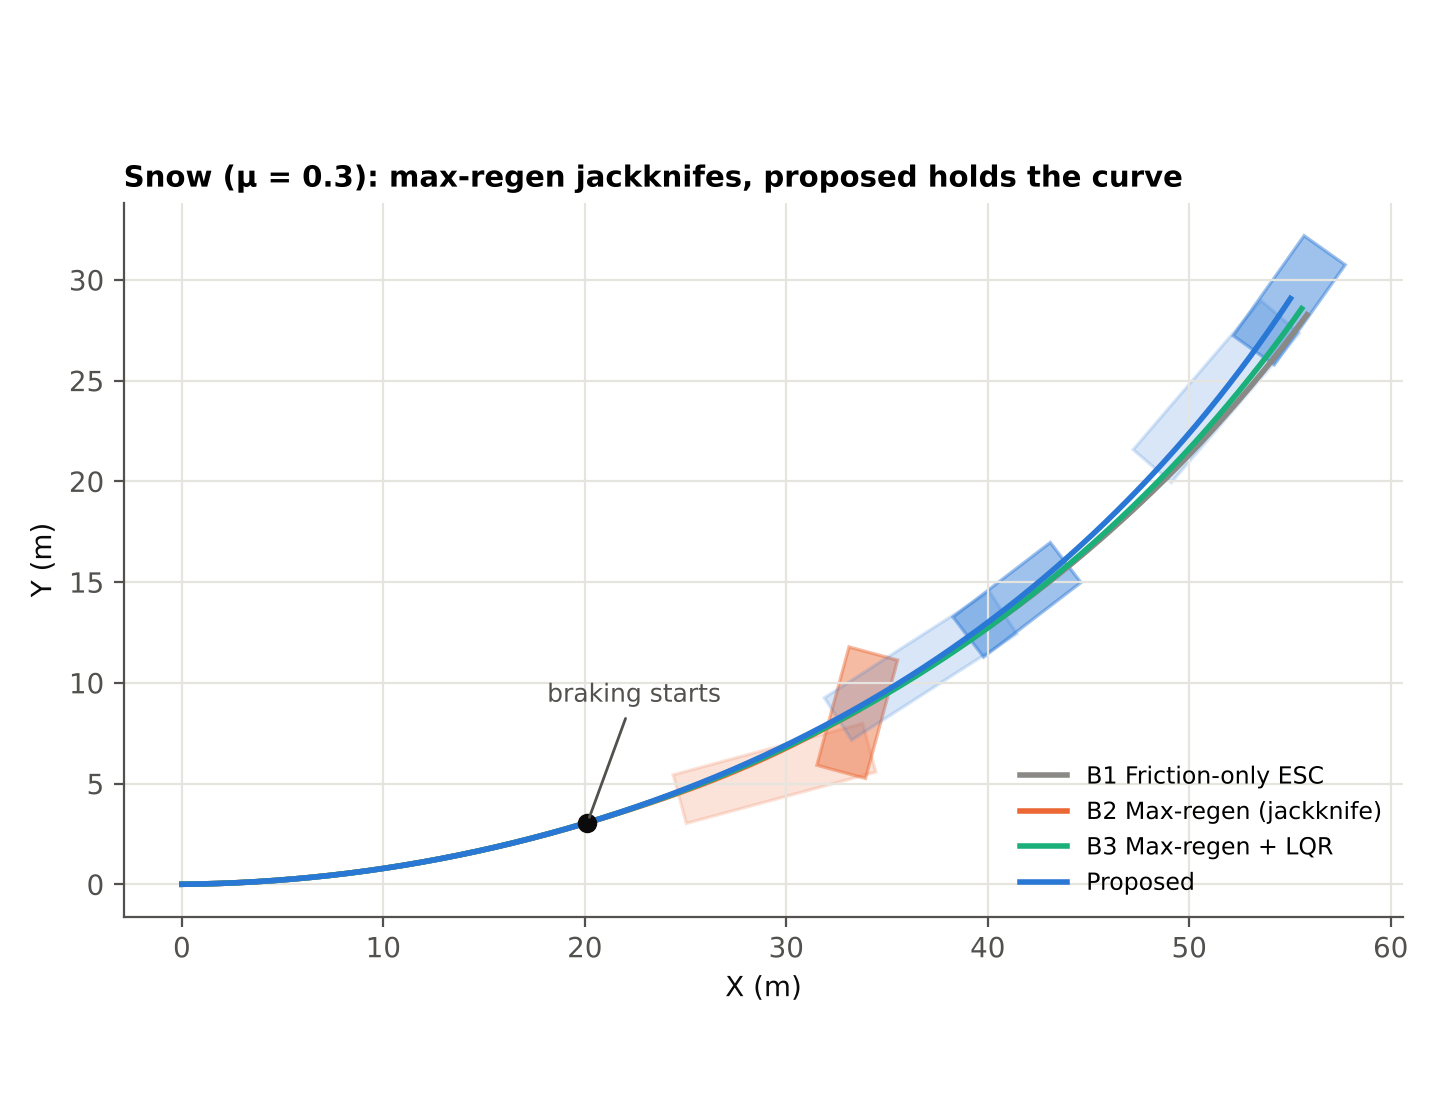
\includegraphics[width=0.92\columnwidth]{fig1_paths_mu03.png}
\caption{Paths and vehicle outlines, brake in turn on snow ($\mu=0.3$), light payload. B2 jackknifes; the proposed controller holds the curve.}
\label{fig:paths}
\end{figure}

\begin{figure}[t]
\centering
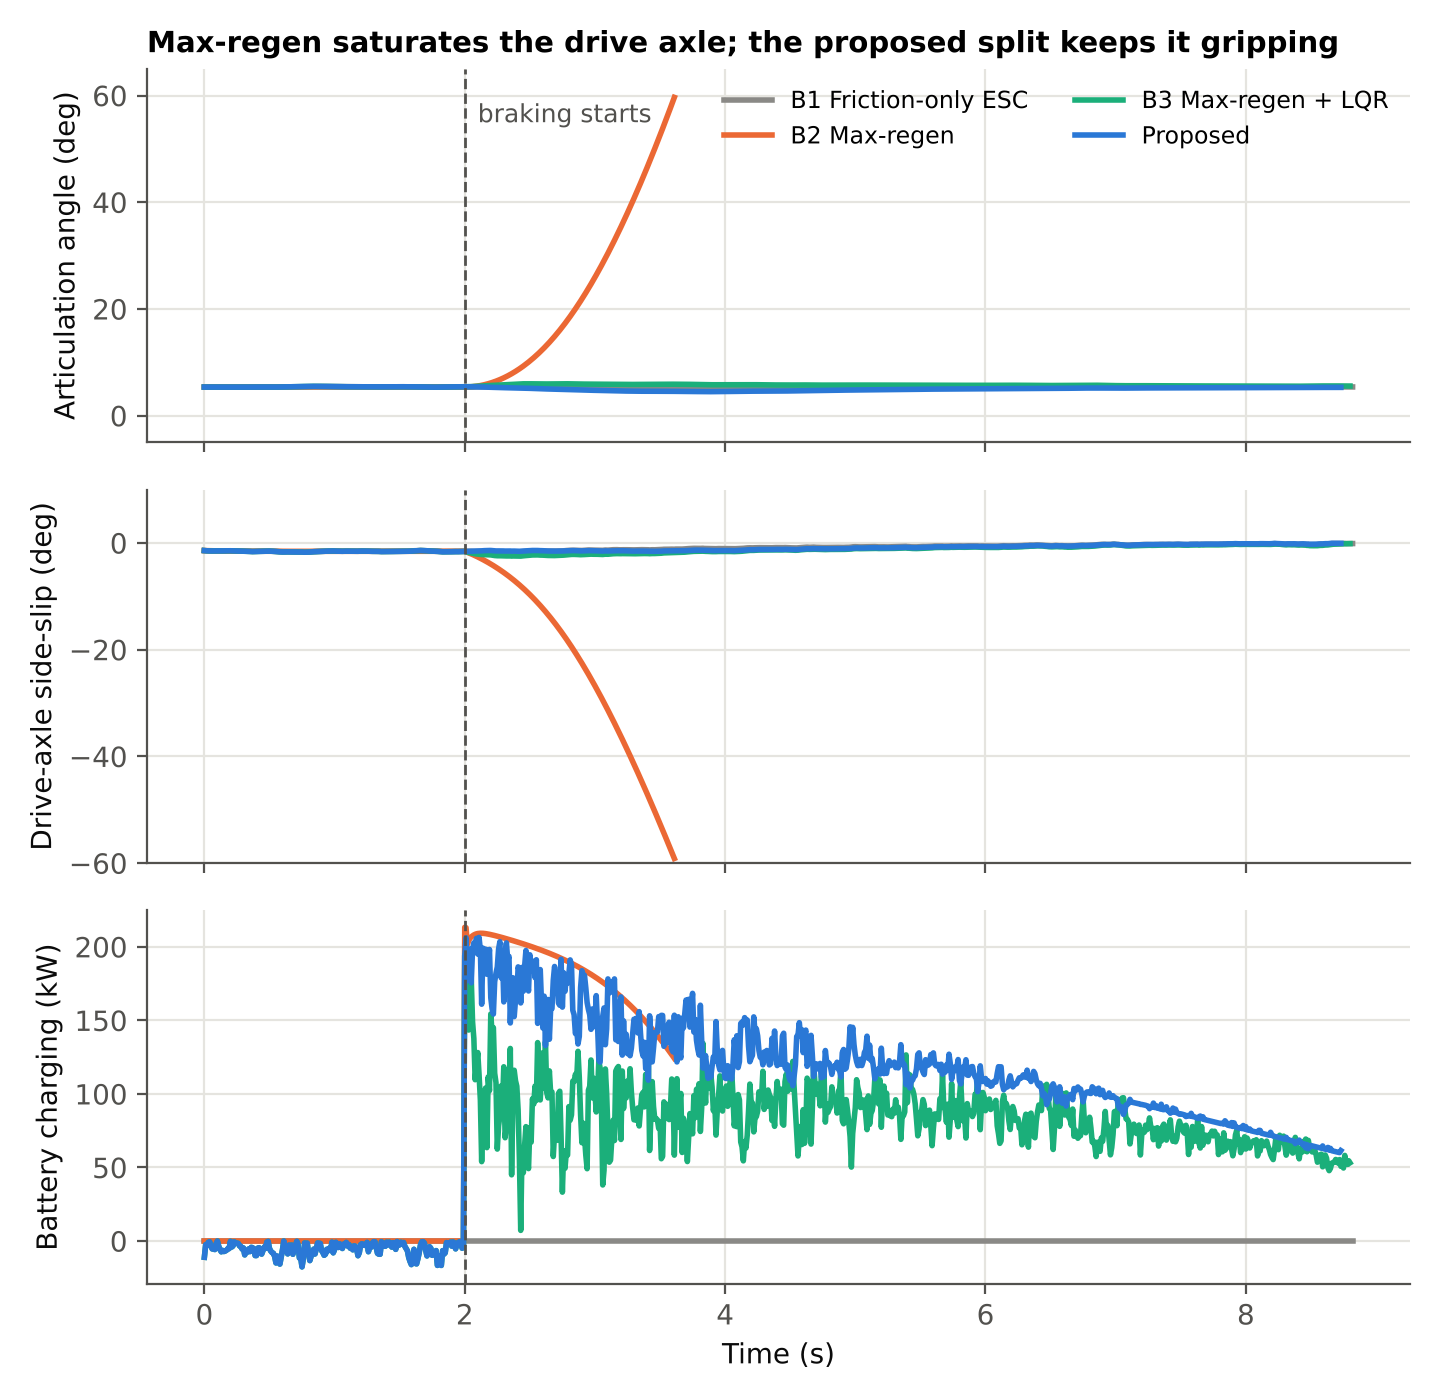
\includegraphics[width=0.92\columnwidth]{fig2_timehist_mu03.png}
\caption{Time histories for the run of Fig.~\ref{fig:paths}. B2 drives the drive axle into saturation; B3 is stable but charges at roughly half the proposed controller's power.}
\label{fig:timehist}
\end{figure}

\begin{table}[t]
\caption{Brake in Turn: Regen Share (\%); \textbf{bold} = Unstable}
\label{tab:bit}
\centering
\begin{tabular}{@{}llrrrr@{}}
\toprule
$\mu$ & Payload & B1 & B2 & B3 & Proposed\\
\midrule
\multirow{3}{*}{0.3} & 13.5 t & 0.0 & \textbf{85.0} & 47.3 & 73.1\\
 & 30 t & 0.0 & \textbf{85.0} & 53.7 & 77.1\\
 & 39 t & 0.0 & \textbf{84.6} & 56.0 & 74.7\\
\midrule
\multirow{3}{*}{0.6} & 13.5 t & 0.0 & \textbf{76.8} & 50.4 & 69.6\\
 & 30 t & 0.0 & \textbf{57.4} & 54.0 & 53.0\\
 & 39 t & 0.0 & 48.7 & 48.2 & 44.1\\
\midrule
\multirow{3}{*}{0.9} & 13.5 t & 0.0 & 63.7 & 59.0 & 57.4\\
 & 30 t & 0.0 & 39.6 & 39.7 & 36.4\\
 & 39 t & 0.0 & 32.4 & 32.4 & 29.6\\
\midrule
\multicolumn{2}{@{}l}{Unstable runs} & 0/9 & 5/9 & 0/9 & 0/9\\
\bottomrule
\end{tabular}
\end{table}

\subsection{Energy Recovery and Ablation}
B2's regen shares on low friction are not usable, because they end in instability. Among the stable controllers, the proposed controller returned 73.1, 77.1 and 74.7\% of the braking energy on snow for the three payloads, against 47.3, 53.7 and 56.0\% for B3, a gain of 19--26 percentage points (Fig.~\ref{fig:regen}); for the light payload this is \SI{0.80}{MJ} against \SI{0.58}{MJ} in one stop from \SI{37}{km/h}.

\begin{figure*}[t]
\centering
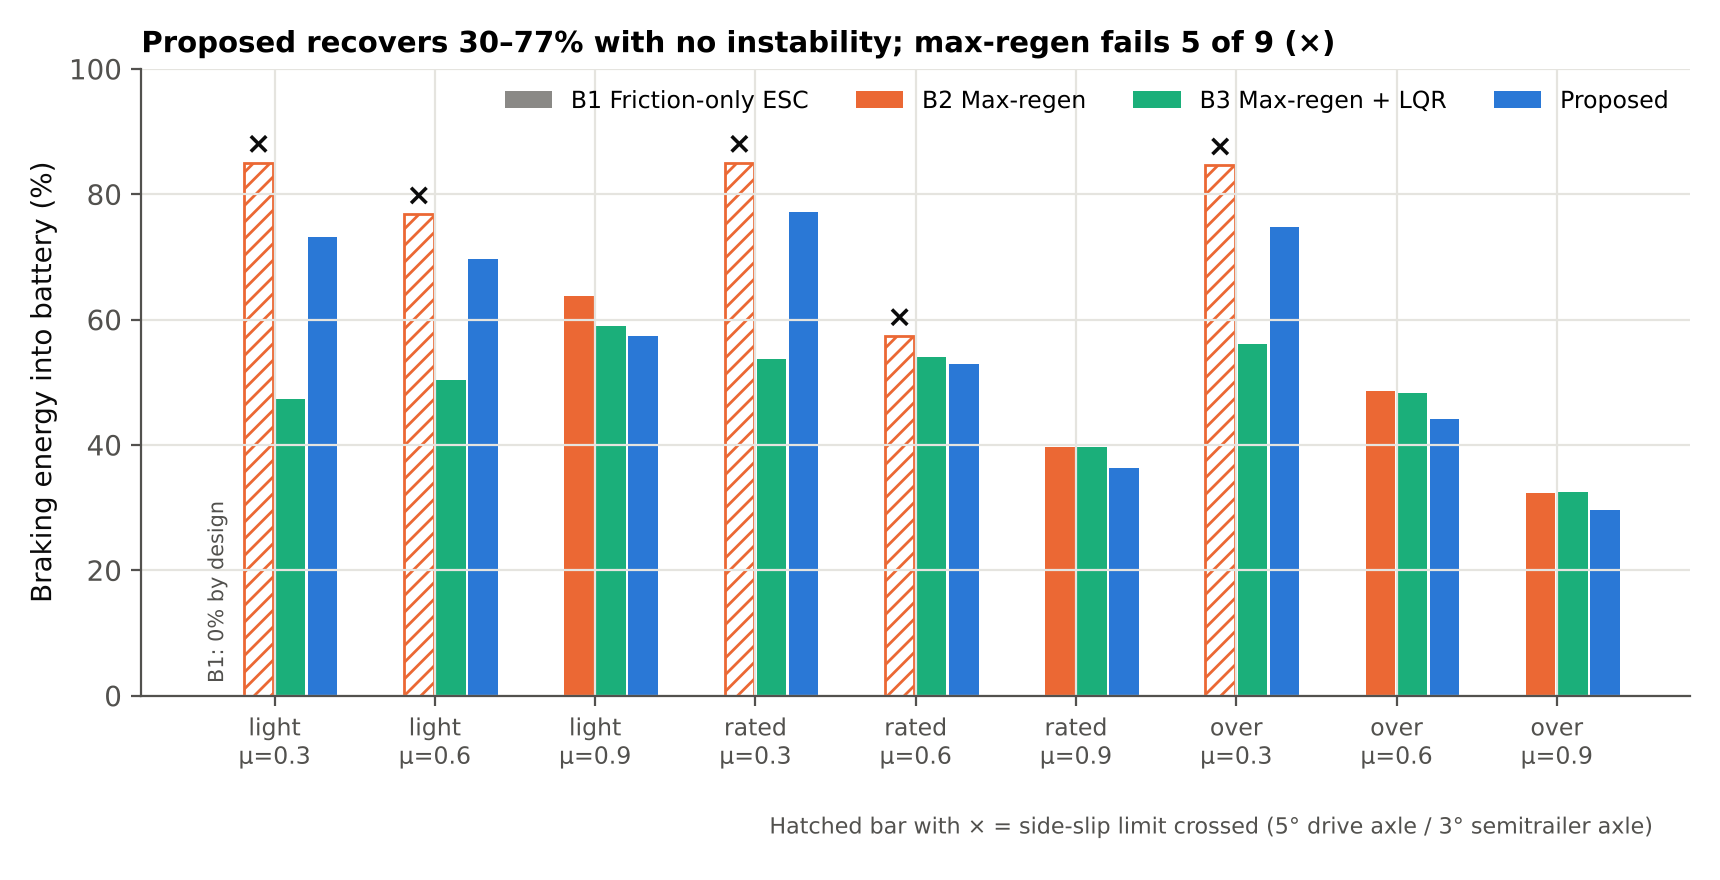
\includegraphics[width=0.8\textwidth]{fig3_regen_by_case.png}
\caption{Share of braking energy returned to the battery in the nine brake-in-turn cases. Hatched bars marked $\times$ crossed a side-slip limit.}
\label{fig:regen}
\end{figure*}

The ablation explains the gain. B3 has the same LQR and filter as the proposed controller but still brakes the drive axle as hard as possible. The tractor begins to yaw, the LQR demands a corrective tractor moment, and because the tractor's single motor with an open differential cannot brake left and right differently, the moment must come from friction brakes, which displace regeneration. B3's peak yaw-moment demand on snow was 40.1--\SI{51.2}{kN\,m}, against 18.9--\SI{19.2}{kN\,m} for the proposed controller. The proposed allocator prevents the yaw disturbance rather than correcting it, so LQR feedback alone prevents jackknife but does not recover the energy.

The cost of the safety margin is small where it exists. In the four cases where B2 remained stable, the proposed controller recovered 2.8--6.3 points less energy. At $\mu\ge0.6$ with the rated or overloaded payload, and at $\mu=0.9$ with the light payload, B3 recovered 1--4 points more than the proposed controller without losing stability: the fixed safety factors bind when they need not, which motivates friction-adaptive caps. Regen share falls with friction for all controllers because the demanded braking power grows with $\mu$ while motor and battery power limits stay fixed. Fig.~\ref{fig:tradeoff} summarises the trade-off: the proposed controller occupies the safe, high-energy region.

\begin{figure}[t]
\centering
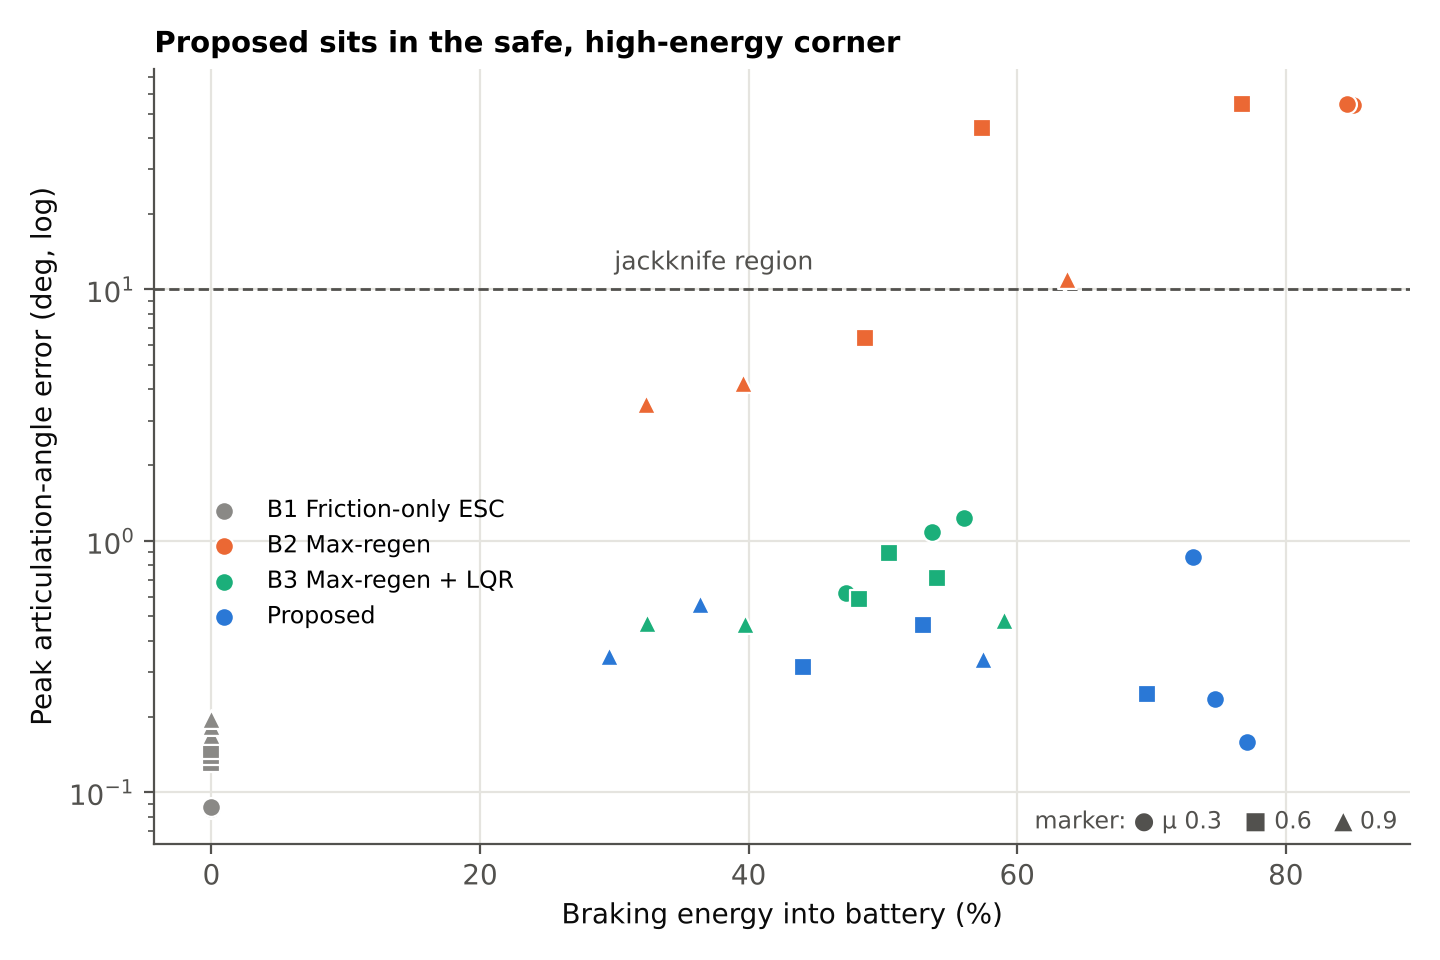
\includegraphics[width=\columnwidth]{fig4_tradeoff.png}
\caption{Stability--energy trade-off over all brake-in-turn runs: energy to the battery against peak articulation error (log scale).}
\label{fig:tradeoff}
\end{figure}

\subsection{Braked Lane Change}
No controller crossed a stability limit in the 24 lane-change runs, and RWA stayed between 0.88 and 1.00 (0.92--0.97 for the proposed controller). The proposed controller recovered 29--65\% of the braking energy, against 33--83\% for B2 and 2--8 points less than B3, and kept the peak articulation error to 0.9--\ang{1.9}, against 2.0--\ang{4.1} for B2. In mild manoeuvres the caps therefore cost energy without a stability benefit, the same conservatism observed at high friction.

\subsection{Robustness}
\label{sec:robust}
Table~\ref{tab:robust} lists the sensitivity runs. The one failure of the proposed controller came from over-estimating the payload: assuming 39~t for a 13.5~t semitrailer on snow, the allocator believed the semitrailer axle could carry more braking than it could, and the semitrailer side-slip changed by \ang{4.26}, beyond the \ang{3} limit. Under-estimating the payload was safe but cost energy (58.4\% against 74.7\% for the correctly known 39~t payload). A payload estimate from air-suspension load sensing or recursive least squares~\cite{vahidi2005}, biased low, is therefore part of the design rather than an add-on. With the yaw-rate gyro alone (four-state filter) the controller remained stable, consistent with the detectability result; it recovered more energy on snow (81.8\%) because the less informed filter demanded smaller moments (peak \SI{4.7}{kN\,m}), at the cost of a larger articulation error (\ang{1.2}). With the battery limited to \SI{100}{kW} the proposed controller remained stable while B2 still jackknifed on snow, showing that the stability comes from the allocation, not from the power limit. Two further noise seeds changed the snow result by under one point.

\begin{table}[t]
\caption{Sensitivity Runs (Proposed Controller Unless Noted)}
\label{tab:robust}
\centering
\begin{tabular}{@{}p{3.0cm}llc@{}}
\toprule
Case & $\mu$ & $\regen$ (\%) & Stable\\
\midrule
Nominal, 13.5 t & 0.3 & 73.1 & yes\\
39 t, assumed 13.5 t & 0.3/0.6/0.9 & 58.4/43.6/31.5 & yes\\
13.5 t, assumed 39 t & 0.3 & 67.7 & \textbf{no}$^{a}$\\
13.5 t, assumed 39 t & 0.6/0.9 & 69.9/57.5 & yes\\
Gyro only & 0.3/0.6/0.9 & 81.8/68.0/56.7 & yes\\
Battery \SI{100}{kW} & 0.3/0.6/0.9 & 49.4/20.9/14.0 & yes\\
Battery \SI{100}{kW}, B2 & 0.3 & 43.6 & \textbf{no}$^{b}$\\
Noise seeds 2, 3 & 0.3 & 73.7, 72.8 & yes\\
\bottomrule
\multicolumn{4}{@{}l}{\footnotesize $^{a}$Semitrailer side-slip change \ang{4.26} $>$ \ang{3}. $^{b}$Jackknife.}
\end{tabular}
\end{table}

\begin{figure}[t]
\centering
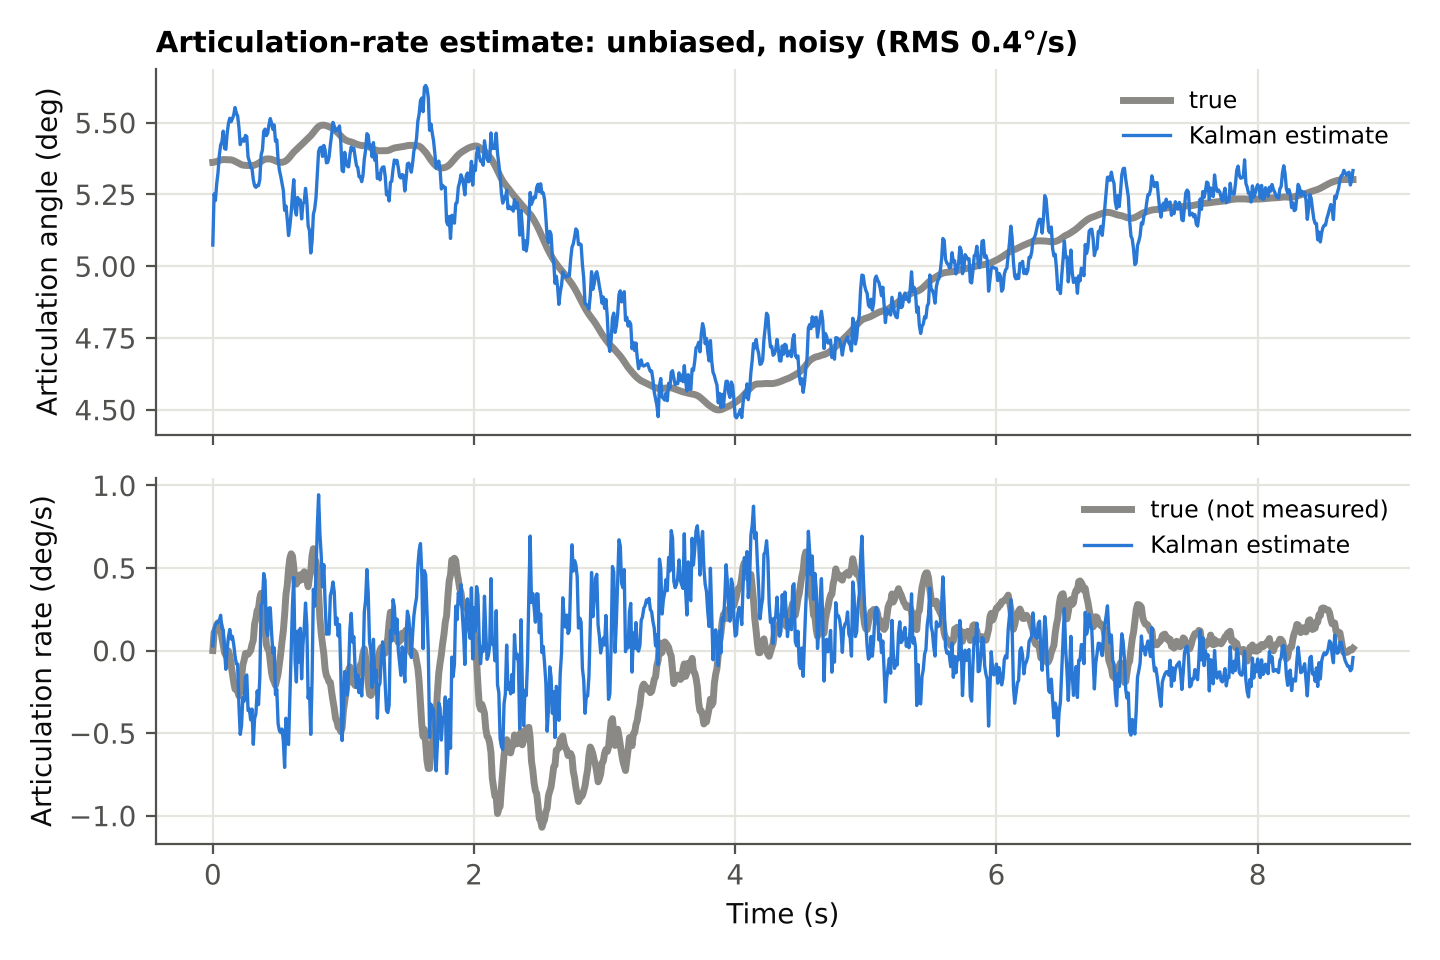
\includegraphics[width=\columnwidth]{fig6_kalman.png}
\caption{Augmented Kalman filter, proposed controller, brake in turn on snow. The articulation rate is not measured; the estimate follows the true value after brake onset.}
\label{fig:kf}
\end{figure}

\subsection{Why Semitrailer-First Allocation Works}
Braking the semitrailer harder than its load share keeps the coupling in tension: the trailer pulls back on the tractor and resists the tractor rotating towards it, as reflected by the $c_1\sin\varphi\,F_{xt}$ term of the equations of motion and consistent with the observation in~\cite{erdinc2023} that semitrailer braking permits more tractor braking without jackknife. Semitrailer braking also preserves the drive-axle load (Section~II-C), and the semitrailer axle carries most of the load for the rated and overloaded cases, so it can absorb most of the regeneration. The risk moves to trailer swing, which the semitrailer cap and the LQR's trailer moment contain, provided the payload is not over-estimated.

\subsection{Limitations}
The study is simulation-only: the models are verified, not validated against measured data, and the motor, battery and payload-scaled semitrailer parameters are representative. The model is planar, without roll or lateral load transfer, so rollover is excluded by limiting lateral acceleration. Axles are lumped, slip control is ideal, and brake and motor dynamics are neglected. Road friction, speed and deceleration are assumed known, and aerodynamic drag, rolling resistance and grade are omitted, which makes the energy shares slightly optimistic. The safety factors were set by judgement, not optimised, and stability of the gain-scheduled LQG loop is shown by simulation rather than proof.

%======================================================================
\section{Conclusion}
An electrified semitrailer can return most of the braking energy on snow without jackknifing, provided the brake allocation is designed around yaw stability. This paper combined a gain-scheduled LQR on both units, a disturbance-augmented Kalman filter and a semitrailer-first, friction-circle-capped regenerative brake allocator, and evaluated them on a nonlinear Lagrangian tractor--semitrailer model over 77 simulations. Energy-first allocation was unstable in 5 of 9 brake-in-turn cases, four of them full jackknifes. The proposed controller was stable in all 15 nominal manoeuvres, recovered 73--77\% of the braking energy on snow, 19--26 points more than the same LQR with energy-first allocation, and gave up only 2.8--6.3 points against maximum regeneration where that was stable. The ablation shows that the allocation, not the yaw feedback alone, recovers the energy on low friction. The design's weak point is payload: over-estimating the semitrailer load made the trailer swing on snow, so the payload estimate must be reliable and biased low.

Future work will make the caps friction-adaptive or replace the rule-based allocator with a constrained model predictive controller that decides allocation and yaw moments jointly with preview of the road, place an online payload and friction estimator in the loop, add roll dynamics and lateral load transfer for rollover-aware caps, and test the allocator in hardware-in-the-loop with real motor and brake dynamics.

%======================================================================
\begin{thebibliography}{99}

\bibitem{erdinc2023}
U.~Erdinc, M.~Jonasson, M.~Sadeghi~Kati, B.~Jacobson, J.~Fredriksson, and L.~Laine, ``Modelling of articulated heavy vehicles for computation of accurate safe operating envelope for yaw stability,'' \emph{Technology Convergence}, 2023. [Online]. Available: https://research.chalmers.se/publication/538592

\bibitem{erdinc2024thesis}
U.~Erdin\c{c}, ``Safe distributed control allocation for articulated heavy vehicles,'' Licentiate thesis, Chalmers Univ.\ of Technology, Gothenburg, Sweden, 2024.

\bibitem{erdinc2024avec}
U.~Erdinc, M.~Jonasson, M.~Sadeghi~Kati, L.~Laine, B.~Jacobson, and J.~Fredriksson, ``Yaw stability control of vehicles using a slip polytope validated with real tests,'' in \emph{Proc.\ AVEC 2024}, Lecture Notes in Mechanical Engineering. Cham, Switzerland: Springer, 2024, doi: 10.1007/978-3-031-70392-8\_19.

\bibitem{bai2020}
Z.~Bai, Y.~Lu, and Y.~Li, ``Method of improving lateral stability by using additional yaw moment of semi-trailer,'' \emph{Energies}, vol.~13, no.~23, Art.~no.~6317, 2020.

\bibitem{vignati2020}
M.~Vignati, S.~Dave, and F.~Cheli, ``Active stabilization of a car--trailer system by means of torque vectoring,'' \emph{Int.\ J.\ Vehicle Systems Modelling and Testing}, 2020.

\bibitem{hou2022}
Hou and Xu, ``High-speed lateral stability and trajectory tracking performance for a tractor-semitrailer with active trailer steering,'' \emph{PLOS ONE}, 2022, doi: 10.1371/journal.pone.0277358.

\bibitem{deng2026}
Deng \emph{et al.}, ``LQR active steering and LTVMPC yaw torque control for distributed drive electric tractor-semitrailer,'' \emph{Proc.\ Inst.\ Mech.\ Eng., Part D: J.\ Automobile Eng.}, 2026, doi: 10.1177/09544070251406651.

\bibitem{vahidi2005}
A.~Vahidi, A.~Stefanopoulou, and H.~Peng, ``Recursive least squares with forgetting for online estimation of vehicle mass and road grade: Theory and experiments,'' \emph{Vehicle System Dynamics}, 2005, doi: 10.1080/00423110412331290446.

\bibitem{ivanov2015}
V.~Ivanov, D.~Savitski, and B.~Shyrokau, ``A survey of traction control and antilock braking systems of full electric vehicles with individually controlled electric motors,'' \emph{IEEE Trans.\ Veh.\ Technol.}, 2015, doi: 10.1109/TVT.2014.2361860.

\bibitem{rajamani2012}
R.~Rajamani, \emph{Vehicle Dynamics and Control}, 2nd~ed. New York, NY, USA: Springer, 2012.

\bibitem{doyle1978}
J.~C.~Doyle, ``Guaranteed margins for LQG regulators,'' \emph{IEEE Trans.\ Autom.\ Control}, 1978, doi: 10.1109/TAC.1978.1101812.

\end{thebibliography}

\end{document}
